\documentclass[11pt,a4paper]{article}

\usepackage{fontspec}
\usepackage{polyglossia}
\setdefaultlanguage{spanish}
\usepackage[margin=2.3cm]{geometry}
\usepackage{graphicx}
\usepackage{booktabs}
\usepackage{tabularx}
\usepackage{longtable}
\usepackage{amsmath}
\usepackage{xcolor}
\usepackage{titlesec}
\usepackage{float}
\usepackage{pdfpages}
\usepackage{url}
\usepackage{caption}
\usepackage{hyperref}

\definecolor{udacolor}{RGB}{0, 102, 51}
\hypersetup{
    colorlinks=true,
    linkcolor=udacolor,
    citecolor=blue,
    urlcolor=blue,
    pdftitle={Informe Práctica 4 - PCB 2 (OBC y ADCS) - CubeSat UD34},
}
\urlstyle{same}
\setlength{\emergencystretch}{3em}

\titleformat{\section}{\Large\bfseries\color{udacolor}}{\thesection.}{1em}{}
\titleformat{\subsection}{\large\bfseries}{\thesubsection.}{1em}{}

\begin{document}

\begin{titlepage}
    \centering
    \vspace*{2cm}
    {\Huge \textbf{\color{udacolor} Universidad de Antioquia}}\\[0.5cm]
    {\LARGE Facultad de Ingeniería}\\[0.5cm]
    {\Large Departamento de Ingeniería Electrónica y Telecomunicaciones}\\[2cm]
    {\huge \textbf{Práctica 4: Diseño Electrónico y Captura Esquemática del CubeSat UD34}}\\[0.6cm]
    {\Large PCB 2 --- Aviónica (OBC) y control de actitud (ADCS)}\\[2cm]
    {\Large \textbf{Integrantes:}}\\[0.5cm]
    {\large Juan Pablo González Blandón --- juan.gonzalez57@udea.edu.co}\\[0.2cm]
    {\large Santiago Castaño Loaiza --- santiago.castano2@udea.edu.co}\\[2cm]
    {\Large \textbf{Curso:}}\\[0.3cm]
    {\large Laboratorio de Diseño de Productos Electrónicos}\\[1cm]
    {\large Proyecto Altium: \texttt{PCB2\_OBC\_ADCS.PrjPcb} (Altium Designer 26.9.1)}\\
    \vfill
    {\large Medellín, Colombia --- 27 de octubre de 2026}
\end{titlepage}

\tableofcontents
\newpage

%%%%%%%%%%%%%%%%%%%%%%%%%%%%%%%%%%%%%%%%%%%%%%%%%%%%%%%%%%%%%%%%
\section{Resumen del estado de la entrega}

Este informe documenta el diseño \textbf{tal como quedó capturado} en el esquemático entregado (cinco hojas: \texttt{Top\_Level}, \texttt{U\_OBC\_Core}, \texttt{U\_Mass\_Storage}, \texttt{U\_ADCS\_Isolated} y \texttt{U\_Interfaces\_Connectors}). Donde el esquemático difiere de lo previsto en la Práctica 3 o en una versión anterior del informe, la diferencia se declara como \emph{desviación} (Sección~\ref{sec:desv}) y no se oculta.

Resultado de la verificación: el error fatal de la compilación (\emph{Missing Harness Type on Signal Harness}), los designadores duplicados y el nombre de red duplicado \texttt{FMC\_SDNE0} fueron corregidos. \textbf{Persisten} los mensajes de \emph{Net has only one pin} y \emph{floating input pins} en \texttt{U\_Mass\_Storage}, porque las señales FMC, SDIO y DCMI no están conectadas a pines del STM32H753. Se aceptan como excepción documentada (sin desactivar el ERC) y se listan como trabajo pendiente para la siguiente revisión. En consecuencia, \textbf{el esquemático no está eléctricamente completo} y no debe considerarse listo para fabricación.

Los cálculos, la BOM, los costos y la matriz de restricciones están en la hoja de cálculo \texttt{UD34\_PCB2\_Calculos\_BOM\_Costos.xlsx} (anexa en el repositorio); las tablas de este informe se generaron a partir de ella para mantener la coherencia.

%%%%%%%%%%%%%%%%%%%%%%%%%%%%%%%%%%%%%%%%%%%%%%%%%%%%%%%%%%%%%%%%
\section{Alcance y especificaciones de la tarjeta}

\subsection{Funciones asignadas}
La PCB 2 es el núcleo de procesamiento y determinación de actitud del nanosatélite UD34. Sus funciones, según la arquitectura de la Práctica 3, son:
\begin{itemize}
    \item \textbf{Procesamiento de datos (OBC):} ejecución de un RTOS, orquestación de DMA para el volcado de imágenes y empaquetamiento de datos. El software no se implementa en esta práctica; el hardware debe ofrecer los recursos necesarios.
    \item \textbf{Almacenamiento masivo:} SDRAM externa por FMC como búfer de ráfaga y eMMC por SDIO como registro de misión.
    \item \textbf{Control de actitud (ADCS):} generación de señales PWM hacia un puente H que excita las bobinas (magnetorquers). \emph{En este esquemático se implementan dos ejes (X e Y)}; la adquisición inercial (IMU) y el eje Z quedan pendientes (desviaciones D-04 y D-05).
\end{itemize}

\subsection{Interfaces con el resto del CubeSat}
La Tabla~\ref{tab:interfaces} resume las interfaces tal como existen en el esquemático. Los conectores son símbolos genéricos de cabecera; no se ha seleccionado aún el conector PC/104 ni el mezzanine previstos en la arquitectura (D-12).

\begin{table}[H]
\centering
\small
\renewcommand{\arraystretch}{1.2}
\begin{tabularx}{\textwidth}{|l|l|X|}
\hline
\textbf{Conector} & \textbf{Hoja} & \textbf{Señales (según esquemático)} \\ \hline
J2 (\texttt{J\_EPS}), 3 pines & Interfaces & 1: \texttt{MAIN\_BUS\_POWER}; 2: \texttt{3V3\_DIGITAL}; 3: \texttt{DGND} \\ \hline
P1 (\texttt{J\_PAYLOAD}), 5 pines & Interfaces & 1: \texttt{SPI\_NSS}; 2: \texttt{SPI\_SCK}; 3: \texttt{SPI\_MISO}; 4: \texttt{SPI\_MOSI}; 5: \texttt{DGND} \\ \hline
P2 (\texttt{J\_CAMERA}), 16 pines & Interfaces & 1--8: \texttt{D0}--\texttt{D7}; 9: \texttt{PCLK}; 10: \texttt{HSYNC}; 11: \texttt{VSYNC}; 12: \texttt{I2C\_SDA}; 13: \texttt{I2C\_SCL}; 14: \texttt{3V3\_DIGITAL}; 15, 16: \texttt{DGND} \\ \hline
P3 (\texttt{J\_TELEM}), 4 pines & Interfaces & 1: \texttt{DGND}; 2: \texttt{3V3\_DIGITAL}; 3: \texttt{I2C\_SCL}; 4: \texttt{I2C\_SDA} (orden a confirmar en el símbolo) \\ \hline
J3 (\texttt{J\_COIL\_X}), 2 pines & Interfaces & \texttt{AOUT1}, \texttt{AOUT2} \\ \hline
J4 (\texttt{J\_COIL\_Y}), 2 pines & Interfaces & \texttt{BOUT1}, \texttt{BOUT2} \\ \hline
J1 (\texttt{53259-0429}), 4 pines & OBC\_Core & \texttt{3V3\_DIGITAL}, \texttt{SWCLK}, \texttt{SWDIO}, \texttt{DGND} (depuración SWD) \\ \hline
\end{tabularx}
\caption{Conectores del esquemático entregado.}
\label{tab:interfaces}
\end{table}

\subsection{Cambio documentado respecto de la Práctica 3: aislamiento galvánico}
La conmutación de las bobinas (corrientes del orden de 1--1{,}5~A) puede inducir ruido en la referencia de tierra y afectar al microcontrolador y a la memoria. Se adoptó un \textbf{aislamiento galvánico digital}: un aislador capacitivo (ISO7741) separa \texttt{DGND} (lado del microcontrolador) de \texttt{PGND} (lado del puente H DRV8833).
\begin{itemize}
    \item \textbf{Ventajas:} desacopla el retorno de potencia del dominio digital; el aislador capacitivo no sufre la degradación por daño de desplazamiento propia de los optoacopladores en entornos de radiación \cite{nasa_sst}.
    \item \textbf{Costos:} más área de tarjeta, más consumo y un convertidor DC-DC aislado para el lado de potencia (previsto: DCP010505BP). \emph{Este convertidor no está capturado en el esquemático} (D-03).
\end{itemize}

%%%%%%%%%%%%%%%%%%%%%%%%%%%%%%%%%%%%%%%%%%%%%%%%%%%%%%%%%%%%%%%%
\section{Selección de componentes}

Se priorizan componentes comerciales (COTS). Su uso no implica calificación para vuelo espacial; el alcance académico del proyecto lo declara explícitamente. La Tabla~\ref{tab:comp} recoge los componentes principales \emph{del esquemático}, las alternativas consideradas y la justificación.

\begin{table}[H]
\centering
\small
\renewcommand{\arraystretch}{1.25}
\begin{tabularx}{\textwidth}{|p{2.2cm}|p{3.0cm}|p{3.0cm}|X|}
\hline
\textbf{Función} & \textbf{Seleccionado} & \textbf{Alternativas} & \textbf{Justificación y puntos por verificar} \\ \hline
Procesamiento & STM32H753IIT6 (LQFP-176) & STM32H743, STM32H750 & Cortex-M7 a 480~MHz, 2~MB de Flash y 1~MB de RAM; periféricos FMC, SDMMC, DCMI, SPI e I\textsuperscript{2}C necesarios para el sistema. Frecuencia final y consumo dependen de la carga de software. \\ \hline
SDRAM & Micron MT48LC4M16A2P-6A (64~Mbit, 3{,}3~V, TSOP-II 54) & ISSI IS42S16400J (previsto en versión anterior) & Interfaz SDRAM síncrona de 16 bits compatible con FMC. Los distribuidores la muestran como \emph{Last Time Buy} con fecha 30/06/2026 ya vencida: la disponibilidad es un riesgo y debe evaluarse una alternativa. \\ \hline
Memoria no volátil & Kingston EMMC04G-M627-A01 (4~GB, FBGA-153) & Otras eMMC 4~GB & VCC 2{,}7--3{,}6~V; en el esquemático \texttt{VCC} y \texttt{VCCQ} están a 3{,}3~V (la versión anterior del informe suponía VCCQ de 1{,}8~V). Encapsulado BGA que condiciona el apilamiento (Sección~\ref{sec:fab}). \\ \hline
Aislamiento digital & TI ISO7741DWR (SOIC-16 DW, 5~kV\textsubscript{rms}) & ISO7740 (4 canales en el mismo sentido) & Tiene 3 canales en un sentido y 1 en el contrario: \textbf{solo caben tres de las cuatro señales PWM}. Para las cuatro señales hace falta el ISO7740 (D-02). \\ \hline
Puente H & TI DRV8833PWPR (HTSSOP-16) & DRV8837, DRV8871 & Dos puentes H, \texttt{VM} 2{,}7--10{,}8~V; cubre dos bobinas. La corriente utilizable depende de la bobina, de \texttt{VM} y de la disipación térmica; no se ha calculado porque no se definió la resistencia de las bobinas. \\ \hline
Reloj HSE & Abracon ABM3B-25.000MHZ-B4U-T & --- & Cristal de 25~MHz para el oscilador del STM32. La capacitancia de carga debe verificarse (Sección~\ref{sec:calc}). \\ \hline
IMU & \emph{No incluida} (previsto ICM-20948) & --- & Referencia en estado EOL según el fabricante; pendiente (D-04). \\ \hline
DC-DC aislado & \emph{No incluido} (previsto DCP010505BP, 1~W) & --- & No sirve para alimentar las bobinas por su potencia; solo para el lado aislado lógico (D-03). \\ \hline
\end{tabularx}
\caption{Componentes principales del esquemático y alternativas.}
\label{tab:comp}
\end{table}

\paragraph{Componentes pasivos y de soporte.} Se usan resistencias de 0603 (10~k$\Omega$ para \texttt{BOOT0}, 4{,}7~k$\Omega$ para \emph{pull-ups} I\textsuperscript{2}C, 33~$\Omega$ en serie en las cuatro líneas SPI), condensadores cerámicos 0402/0603 para el reloj, \texttt{VCAP} y reinicio, y los conectores de la Tabla~\ref{tab:interfaces}. Para las referencias exactas véase la BOM (Sección~\ref{sec:bom}).

%%%%%%%%%%%%%%%%%%%%%%%%%%%%%%%%%%%%%%%%%%%%%%%%%%%%%%%%%%%%%%%%
\section{Diseño y dimensionamiento de circuitos}\label{sec:calc}

Los cálculos están en la hoja \texttt{Calculos} del libro de cálculo; aquí se resumen con sus supuestos.

\subsection{Alimentación y dominios}
El dominio lógico es \texttt{3V3\_DIGITAL}, que llega al STM32, a la SDRAM, a la eMMC, al lado 1 del aislador y a los conectores. En el esquemático, el lado aislado usa la etiqueta \texttt{5V\_ISO} para \texttt{VCC2} del ISO7741 y para \texttt{VM} del DRV8833, pero \textbf{no hay ninguna fuente que genere esa red} (D-03). La versión anterior del informe preveía alimentar el puente H desde $V_{BATT}$ (7{,}4--8{,}4~V) y usar el DCP010505BP solo para el lado aislado lógico; esa arquitectura no está capturada.

El consumo digital heredado del informe anterior (estimado, sin verificar con hojas de datos) es 100~mA nominal y 250~mA pico a 3{,}3~V, es decir, 0{,}33~W y 0{,}825~W ($P=VI$). El consumo de las bobinas no se calcula porque su resistencia no está definida.

\subsection{Red de carga del cristal HSE}
Para dos condensadores iguales, $C_{ext}=2(C_L-C_{stray})$. La versión anterior usaba $C_L=8$~pF y obtenía 12~pF. La referencia seleccionada (ABM3B-25.000MHZ-B4U-T) tiene, según un distribuidor, $C_L=18$~pF (\textbf{por verificar en la hoja de datos de Abracon}). Con $C_{stray}=3$~pF (supuesto) resulta:
\[
C_{ext}=2(18-3)=30\ \mathrm{pF},
\]
mientras que el esquemático instala 16~pF por lado, lo que da una capacitancia de carga efectiva $C_L = 16/2+3 = 11$~pF, 7~pF por debajo de la requerida. Esto puede desviar la frecuencia o afectar el arranque del oscilador. Se registra como desviación D-06 y debe corregirse en la siguiente revisión.

\subsection{Resistencias de polarización de I\textsuperscript{2}C}
Con $V_{CC}=3{,}3$~V, $V_{OL}=0{,}4$~V, $I_{OL}=3$~mA, $t_r=300$~ns y $C_b=50$~pF (supuesto):
\[
R_{p(min)}=\frac{3{,}3-0{,}4}{3\,\mathrm{mA}}\approx 967\ \Omega,\qquad
R_{p(max)}=\frac{300\,\mathrm{ns}}{0{,}8473\cdot 50\,\mathrm{pF}}\approx 7{,}08\ \mathrm{k}\Omega.
\]
Los 4{,}7~k$\Omega$ instalados (R6, R7) están dentro del intervalo. Cumple.

\subsection{Ancho de pista para las bobinas}
Con IPC-2221 para capa externa ($k=0{,}048$, $\Delta T=10$~°C, cobre de 1~oz): $A=(I/(k\,\Delta T^{0{,}44}))^{1/0{,}725}$ y $w=A/(1{,}378\ \mathrm{mil})$. Para 1~A resulta $\approx 0{,}30$~mm y para 1{,}5~A, $\approx 0{,}53$~mm. Como objetivo de diseño se propone $\geq 1$~mm para la potencia, por margen y caída de tensión. El valor de corriente es un supuesto: la corriente real depende de la resistencia de la bobina (no definida).

\subsection{Magnetorquers}
Se mantiene como referencia el momento dipolar $m=NIA_{ef}$ y el par $\boldsymbol{\tau}=\boldsymbol{m}\times\boldsymbol{B}$. No se dimensionan las bobinas en esta entrega (el objetivo de $0{,}07\ \mathrm{A\,m^2}$ por eje es una referencia genérica de 1U y no un requisito confirmado de UD34). Solo hay dos ejes en el esquemático.

\subsection{Arranque, depuración y pines no usados}
\begin{itemize}
    \item \texttt{BOOT0} a \texttt{DGND} mediante 10~k$\Omega$ (R1).
    \item Interfaz SWD de 4 pines (J1: \texttt{3V3\_DIGITAL}, \texttt{SWCLK}, \texttt{SWDIO}, \texttt{DGND}) y condensador de 100~nF en \texttt{NRST}.
    \item Pines no usados del microcontrolador: quedan sin conectar. Para las entradas de periféricos no usados se recomienda configurarlos como analógicos o salida en el firmware.
    \item Puntos de prueba: previstos en la versión anterior (NRST, VCAP, \texttt{3.3V\_Iso}, PWM) pero \textbf{no capturados} (D-10).
    \item Desacoplamiento: el esquemático no incluye un condensador por cada par VDD/VSS del STM32 (D-08).
\end{itemize}

%%%%%%%%%%%%%%%%%%%%%%%%%%%%%%%%%%%%%%%%%%%%%%%%%%%%%%%%%%%%%%%%
\section{Librerías de componentes}

El proyecto usa tres archivos de librería propios en el repositorio (\texttt{Esquematicos/2\_Libraries}): \texttt{UD34\_Sym.SchLib} (símbolos), \texttt{UD34\_Footprints.PcbLib} (huellas) y \texttt{UD34\_Components.LibPkg} (paquete de librerías que resuelve las dependencias). En el proyecto aparecen sin errores de compilación de librería.

\paragraph{Estado de la verificación.} Los símbolos y las huellas se revisan frente a las hojas de datos con la lista siguiente. \textbf{Esta revisión no está documentada de forma completa en esta entrega}; se deja la lista como criterio y queda pendiente registrar el resultado por componente:
\begin{itemize}
    \item nombres, números y tipos eléctricos de los pines del símbolo;
    \item correspondencia pines--pads, incluido el pad térmico del DRV8833 (PowerPAD);
    \item encapsulado exacto, numeración y orientación del pin 1;
    \item patrón de montaje recomendado;
    \item parámetros de fabricante y MPN (que alimentan la BOM).
\end{itemize}
Las hojas de datos disponibles en el repositorio (\texttt{3\_Datasheets}) son las del STM32H753IIT6, MT48LC4M16A2P, ISO7741DWR y DRV8833PWPR. Faltan en el repositorio las del eMMC Kingston, del cristal ABM3B, del conector Molex 53259-0429 y de los pasivos (D-14, ver también Sección~\ref{sec:repo}).

%%%%%%%%%%%%%%%%%%%%%%%%%%%%%%%%%%%%%%%%%%%%%%%%%%%%%%%%%%%%%%%%
\section{Captura esquemática jerárquica}

\subsection{Estructura}
\texttt{Top\_Level.SchDoc} conecta cuatro hojas mediante \emph{Sheet Entries} (señales simples) y \emph{signal harnesses} (buses):
\begin{itemize}
    \item \textbf{U\_OBC\_Core:} STM32H753IIT6, reloj, reinicio, depuración SWD, \emph{pull-ups} I\textsuperscript{2}C y resistencias serie SPI. Define los harness \texttt{FMC\_BUS\_TYPE}, \texttt{SDIO\_BUS\_TYPE}, \texttt{PAYLOAD\_SPI\_TYPE}, \texttt{I2C\_DEF}, \texttt{DCMI\_DEF} y \texttt{ADCS\_CTRL\_DEF}.
    \item \textbf{U\_Mass\_Storage:} SDRAM MT48LC4M16A2P-6A y eMMC EMMC04G-M627.
    \item \textbf{U\_ADCS\_Isolated:} aislador ISO7741DWR y puente H DRV8833PWPR; harness \texttt{COIL\_X\_DEF} y \texttt{COIL\_Y\_DEF}.
    \item \textbf{U\_Interfaces\_Connectors:} conectores y filtrado de la entrada de potencia (C6 de 0{,}1~$\mu$F y C7 de 10~$\mu$F).
\end{itemize}

\subsection{Reutilización}
Los harness (\texttt{.Harness}) definen cada interfaz una sola vez y se comparten entre las hojas, lo que permite reutilizar la interfaz SPI, I\textsuperscript{2}C, DCMI, FMC y SDIO en otras tarjetas. No se identificaron bloques repetidos que justifiquen diseño multicanal; las bobinas X e Y comparten el mismo DRV8833 (dos puentes H).

\subsection{Documentación de las hojas}
Los nombres de red son coherentes entre hojas. \textbf{Los cajetines de las hojas están vacíos} (título, número, revisión, autor); debe completarse antes de la entrega final (D-13).

%%%%%%%%%%%%%%%%%%%%%%%%%%%%%%%%%%%%%%%%%%%%%%%%%%%%%%%%%%%%%%%%
\section{Restricciones de PCB y condiciones de fabricación}\label{sec:fab}

\subsection{Proveedor y capacidades}
Se eligió \textbf{JLCPCB} (fabricación de PCB rígida estándar). Las capacidades se consultaron el 27/10/2026 en \url{https://jlcpcb.com/capabilities/pcb-capabilities} y \url{https://api.jlcpcb.com/capabilities/Capabilities}. Valores relevantes registrados:
\begin{itemize}
    \item Capas: 1 a 32; impedancia controlada desde 4 capas.
    \item Taladro: 0{,}20--6{,}30~mm. Vía en 2 capas: taladro mínimo 0{,}3~mm y diámetro 0{,}5~mm; en multicapa: 0{,}2~mm y 0{,}45~mm.
    \item Separación pista--borde (fresado): 0{,}2~mm. Paso mínimo de pines de CI: 0{,}4~mm.
    \item Guía BGA: vía de abanico con taladro 0{,}15~mm y relleno (POFV) disponible en 6--20 capas.
\end{itemize}
Algunos valores de anchos mínimos y de anillo anular provienen de fuentes secundarias y están marcados \emph{por confirmar} en la matriz. Un valor mínimo de fabricación no garantiza que la geometría sea adecuada para la corriente o la señal; por eso las restricciones eléctricas se derivan aparte.

\subsection{Apilamiento preliminar}
Se propone 4 capas (señal / GND / alimentación / señal), FR-4, 1{,}6~mm, cobre exterior de 1~oz, por la presencia del eMMC en FBGA-153, el microcontrolador de 176 pines, el bus FMC de 38 señales y los dominios aislados. Los valores geométricos que dependen del apilamiento (impedancias, anchos) se definirán en la guía de enrutamiento. Podría ser necesario un servicio especial para el BGA (vía rellena o HDI).

\subsection{Matriz de restricciones}
La Tabla~\ref{tab:matriz} contiene la matriz. Se distingue entre condiciones \emph{exigidas} por una fuente técnica, \emph{recomendaciones} adoptadas por el equipo e \emph{inferencias} propias. Donde la fuente dice \emph{por confirmar}, el valor no se contrastó con la hoja de datos en esta entrega.

\tiny
\setlength{\tabcolsep}{3pt}
\renewcommand{\arraystretch}{1.15}
\begin{longtable}{|>{\raggedright\arraybackslash}p{1.1cm}|>{\raggedright\arraybackslash}p{1.8cm}|>{\raggedright\arraybackslash}p{5.6cm}|>{\raggedright\arraybackslash}p{1.6cm}|>{\raggedright\arraybackslash}p{4.0cm}|>{\raggedright\arraybackslash}p{1.8cm}|}
\hline
\textbf{ID} & \textbf{Origen} & \textbf{Restricción y alcance} & \textbf{Tipo} & \textbf{Fuente y fundamento} & \textbf{Estado} \\ \hline
\endfirsthead
\hline
\textbf{ID} & \textbf{Origen} & \textbf{Restricción y alcance} & \textbf{Tipo} & \textbf{Fuente y fundamento} & \textbf{Estado} \\ \hline
\endhead
PCB-01 & ET alimentación / MAIN\_BUS\_POWER & Pista de MAIN\_BUS\_POWER (J\_EPS pin 1) y VM del DRV8833: ancho mínimo según Calculos B28 ($\approx$0,30 mm para 1 A y $\approx$0,53 mm para 1,5 A, $\Delta$T 10 \textdegree{}C, 1 oz externa); usar $\geq$ 1 mm como objetivo de diseño por margen y caída de tensión. Evitar cuellos de botella en vías: mínimo 2 vías 0,3/0,6 mm por transición. & Inferencia + recomendación & IPC-2221 (cálculo en hoja Calculos); corriente supuesta 1 A (informe previo 1-1,5 A). & Pendiente de layout \\ \hline
PCB-02 & Dominio ADCS aislado & Dominios DGND y PGND separados galvánicamente. Distancia mínima (creepage/clearance) entre copper de DGND y de PGND en la zona del ISO7741: $\geq$ 8 mm de pad a pad en el aislador DW (SOIC-16 ancho) y sin cobre ni planos bajo el aislador en la barrera. & Exigida por componente + recomendación & ISO7741DWR: aislamiento 5000 Vrms (DigiKey/TI). Distancia exacta: hoja de datos TI, sección Package/Insulation Specifications (por confirmar valor numérico). & Pendiente de layout \\ \hline
PCB-03 & Dominio ADCS aislado & El plano/retorno de PGND no debe cruzar ni solaparse con DGND. Un único punto de conexión no existe (aislamiento total); los retornos de las bobinas vuelven a PGND por el lado del DRV8833. & Recomendación & Práctica estándar de aislamiento galvánico; cambio documentado en el informe, Sección 2.3. & Pendiente de layout \\ \hline
PCB-04 & DRV8833 / J\_COIL\_X, J\_COIL\_Y & Pad térmico (PowerPAD) de U4 conectado a PGND con matriz de vías térmicas (mín. 5 vías 0,3 mm de taladro) a plano de PGND. Zona de cobre ampliada alrededor del pad. & Recomendación del fabricante & Hoja de datos DRV8833, sección Layout (PowerPAD) - confirmar número de vías recomendado. & Pendiente de layout \\ \hline
PCB-05 & STM32H753 / alimentación & Un condensador de desacoplamiento de 100 nF por cada par VDD/VSS, a $\leq$ 3 mm del pin, con vía directa al plano. El esquemático actual NO incluye estos condensadores (ver Desviaciones D-08); deben añadirse o compensarse con condensadores en la zona de layout. & Exigida por hoja de datos & AN4938 / datasheet STM32H753 (sección Power supply scheme). Cantidad exacta por confirmar. & Desviación abierta \\ \hline
PCB-06 & STM32H753 / VCAP & Condensadores VCAP (C3, C4 de 2,2 uF) lo más cerca posible de los pines VCAP (81, 125), ESR < 100 mohm (cerámico X7R/X5R). & Exigida por hoja de datos & Datasheet STM32H753, sección Power supply scheme (VCAP). Confirmar valor y ESR. & Pendiente de layout \\ \hline
PCB-07 & Reloj HSE & Cristal Y1 y condensadores C2, C5 juntos, a $\leq$ 5 mm de PH0/PH1; sin pistas de otras señales ni vías bajo el cristal; guarda de GND (DGND) alrededor. & Recomendación del fabricante & AN2867 (Oscillator design guide for STM8/STM32) - confirmar aplicabilidad al H7. & Pendiente de layout \\ \hline
PCB-08 & Reloj HSE & Capacitancia de carga CL = 18 pF (a verificar): requiere Cext $\approx$ 30 pF por lado con Cstray = 3 pF; instalado 16 pF. Desviación abierta. & Exigida por hoja de datos & Hoja de datos ABM3B-25.000MHZ-B4U-T (por confirmar) + Calculos B3-B9. & Desviación abierta \\ \hline
PCB-09 & IF-04 PAYLOAD\_SPI & SPI hacia el payload: resistencias serie de 33 ohm (R2-R5) ubicadas cerca del origen (STM32). Longitud de pista < 100 mm si es posible; sin cruces de planos. & Recomendación & Práctica de integridad de señal; impedancia no controlada en esta etapa. & Pendiente de layout \\ \hline
PCB-10 & IF-05 TELEMETRY\_I2C & Pull-ups de 4,7 kohm (R6, R7) a 3V3\_DIGITAL dentro del intervalo [967 ohm; 7,08 kohm]. & Cálculo & Hoja Calculos B16-B19 (especificación I2C). & Cumple \\ \hline
PCB-11 & IF-01 CAMERA\_DCMI & Bus DCMI (D0-D7, PCLK, HSYNC, VSYNC): grupo de longitud con diferencia máxima entre D0-D7 y PCLK a definir en la guía de enrutamiento (objetivo preliminar $\leq$ 5 mm); referencia continua de plano. & Inferencia (objetivo) & Requisito ET-01 $\geq$ 40 MB/s (informe). Valor numérico por derivar de la hoja de datos de la cámara (no disponible en este paquete). & Pendiente (valor por definir) \\ \hline
PCB-12 & FMC\_BUS (SDRAM) & Bus FMC SDRAM: línea de reloj FMC\_SDCLK emparejada en longitud con el grupo de datos/control (objetivo $\leq$ 10 mm de diferencia); cobertura por plano de referencia; la SDRAM junto al STM32. & Inferencia (objetivo) & Práctica común para SDRAM síncrona (timing del MT48LC4M16A2P-6A, hoja de datos: sección AC Timing). Valores numéricos por confirmar. & Pendiente (valor por definir) \\ \hline
PCB-13 & SDIO\_BUS (eMMC) & Bus SDIO: CLK separado de D0-D7 y CMD; diferencia de longitud entre líneas $\leq$ 5 mm (objetivo); eMMC en BGA FBGA-153: abanico con vías de 0,15-0,2 mm (HDI o POFV según proveedor). & Inferencia + límite de fabricación & Datasheet Kingston EMMC04G-M627-A01 (por confirmar) y guía BGA de JLCPCB (\url{https://jlcpcb.com/help/article/243-BGA-Design-Guidelines---PCB-Layout-Recommendations-for-BGA-packages}). & Pendiente de layout \\ \hline
PCB-14 & SWD (J1) & SWDIO y SWCLK cortos (< 50 mm) hacia el conector J1; NRST disponible en test point. & Recomendación & Práctica; el informe prevé puntos de prueba NRST, VCAP, 3.3V\_Iso y PWM. & Desviación abierta \\ \hline
PCB-15 & Térmico & Disipación del DRV8833 y de las pistas de bobinas: cobre de superficie ampliado y, si se justifica, capa interna de potencia; $\Delta$T admisible 10 \textdegree{}C como objetivo. & Recomendación & Hoja de datos DRV8833; IPC-2221. & Pendiente \\ \hline
PCB-16 & Conectores & J1 (53259-0429) y cabeceras de cables en el borde de la tarjeta; huella de THT con agujeros de taladro según datasheet Molex; pitch 3,5 mm (J1). & Exigida por huella & Datasheet Molex 53259-0429 (patrón recomendado). & Pendiente de verificación \\ \hline
FAB-01 & Proveedor & Proveedor elegido: JLCPCB (fabricación de PCB rígida estándar). Capacidades consultadas el 27/10/2026 en \url{https://jlcpcb.com/capabilities/pcb-capabilities} y \url{https://api.jlcpcb.com/capabilities/Capabilities.} Los valores pueden cambiar; reconsultar antes del pedido. & Fuente externa & JLCPCB, páginas de capacidades (fecha de consulta 27/10/2026). & Documentado \\ \hline
FAB-02 & Apilamiento & Número de capas preliminar: 4 capas (señal / GND / alimentación / señal), FR-4, 1,6 mm, cobre exterior 1 oz (0,035 mm). Justificación: BGA FBGA-153, 176 pines LQFP, bus FMC de 38 señales y dominios aislados. Cálculo de impedancias y apilamiento definitivos quedan para la guía de enrutamiento. & Inferencia & JLCPCB: soporta 1-32 capas, impedancia controlada de 4 capas en adelante, con apilamientos por defecto. & Pendiente (valor preliminar) \\ \hline
FAB-03 & Pistas y separación & Ancho y separación mínimos en capa exterior a usar en diseño: $\geq$ 0,127 mm (5 mil) / 0,127 mm (5 mil) para 1-2 capas; objetivo de diseño $\geq$ 0,15 mm / 0,15 mm para tener margen. En multicapa JLCPCB indica 3,5 mil como límite; no se usa por margen. & Límite de fabricante & JLCPCB capabilities (resumen verificado vía secundaria: Trace width/spacing 5 mil 1-2L; 3,5 mil multicapa). Reconsultar el valor exacto de 4 capas en la página oficial. & Pendiente de layout \\ \hline
FAB-04 & Vías y taladros & Vía estándar: taladro 0,3 mm / diámetro 0,5 mm (2 capas) o taladro 0,2 mm / diámetro 0,45 mm (multicapa); vías de abanico de BGA con taladro 0,15 mm / diámetro 0,25 mm (según la guía BGA y 'Via-in-pad' con relleno, POFV gratuito en 6-20 capas). Taladro mínimo 0,2 mm; máximo 6,3 mm. & Límite de fabricante & JLCPCB capabilities (\url{https://api.jlcpcb.com/capabilities/Capabilities}) y guía BGA (\url{https://jlcpcb.com/help/article/243-BGA-Design-Guidelines---PCB-Layout-Recommendations-for-BGA-packages}). & Pendiente de layout \\ \hline
FAB-05 & Anillo anular / máscara & Anillo anular mínimo de pad $\geq$ 0,15 mm sobre el taladro (valor registrado por fuente secundaria). Puente de máscara de soldadura mínimo según proveedor; verificar para el paso de 0,5 mm del LQFP-176 y del FBGA-153. & Límite de fabricante & JLCPCB (valores a confirmar en la página oficial); la separación mínima entre pines de IC es 0,4 mm (0,35 mm extremo). & Pendiente (confirmar) \\ \hline
FAB-06 & Borde de tarjeta & Distancia de pista a borde $\geq$ 0,2 mm (fresado) como límite del fabricante; objetivo de diseño $\geq$ 0,3 mm. Tamaño de lote en prototipo: tarjeta individual 70x70 mm mínimo / 400x500 mm máximo en el servicio estándar. & Límite de fabricante & JLCPCB capabilities (Trace to Outline 0,2 mm; Single PCB Size). & Pendiente \\ \hline
FAB-07 & Tamaño de la placa & Tamaño de la PCB debe respetar el formato 1U del CubeSat (\textasciitilde{} 90 x 96 mm de la placa PC/104). Si es menor de 70 x 70 mm, verificar los mínimos del servicio estándar de JLCPCB. & Inferencia & Estándar CubeSat 1U / PC/104 (por confirmar en la arquitectura de la práctica 3). & Pendiente \\ \hline
FAB-08 & Servicios especiales & Posible necesidad de servicio especial: vía rellena (POFV/via-in-pad) y/o HDI para el FBGA-153 a paso 0,5 mm; impedancia controlada si se exige. Identificado para consultar a JLCPCB. & Inferencia & Guía BGA de JLCPCB. & Pendiente \\ \hline
\end{longtable}
\normalsize
\captionof{table}{Matriz de restricciones de PCB y fabricación.}\label{tab:matriz}

\subsection{Incorporación al esquemático}
\textbf{No se han creado directivas \emph{Parameter Set} en el esquemático en esta entrega.} Las restricciones están registradas en la matriz y en la hoja \texttt{Restricciones} del libro de cálculo. Quedan como trabajo pendiente: clases de red \texttt{POWER}, \texttt{PGND}, \texttt{FMC}, \texttt{SDIO}, \texttt{DCMI} y \texttt{SPI}, con reglas de ancho (Width) y de separación (Clearance) asociadas; las reglas de longitud de grupo se configurarán en el gestor de restricciones durante el enrutamiento. Las instrucciones de ubicación (desacoplamiento, cristal, vías térmicas) quedan como notas y entradas de la matriz.

%%%%%%%%%%%%%%%%%%%%%%%%%%%%%%%%%%%%%%%%%%%%%%%%%%%%%%%%%%%%%%%%
\section{Verificación del diseño}

\subsection{Revisión automática (ERC)}
Se ejecutó la compilación del proyecto en Altium Designer; el registro está en la Tabla~\ref{tab:erc}.
\tiny
\setlength{\tabcolsep}{3pt}
\renewcommand{\arraystretch}{1.15}
\begin{longtable}{|>{\raggedright\arraybackslash}p{1.5cm}|>{\raggedright\arraybackslash}p{2.0cm}|>{\raggedright\arraybackslash}p{3.2cm}|>{\raggedright\arraybackslash}p{3.3cm}|>{\raggedright\arraybackslash}p{3.9cm}|>{\raggedright\arraybackslash}p{1.8cm}|}
\hline
\textbf{Fecha/hora} & \textbf{Hoja} & \textbf{Mensaje(s)} & \textbf{Causa} & \textbf{Resolución} & \textbf{Estado} \\ \hline
\endfirsthead
\hline
\textbf{Fecha/hora} & \textbf{Hoja} & \textbf{Mensaje(s)} & \textbf{Causa} & \textbf{Resolución} & \textbf{Estado} \\ \hline
\endhead
27/10/2026 06:03 & Top\_Level.SchDoc & [Fatal Error] Missing Harness Type on Signal Harness & Había un tramo de cable de harness suelto fuera del diagrama y Sheet Entries sin Harness Type (TELEMETRY\_I2C, PAYLOAD\_SPI). & Se asignó el Harness Type correcto a los Sheet Entries y se eliminó el cable suelto. & Resuelto \\ \hline
27/10/2026 06:03 & U\_Interfaces\_Connectors / U\_OBC\_Core & Duplicate Component Designators C5, J1; Duplicate Net Names NetC5\_1 & Designadores repetidos entre hojas y eMMC sin anotar ('*'). & Tools > Annotation > Reset All y Annotate Schematics (Across Then Down). & Resuelto \\ \hline
27/10/2026 06:20 & Top\_Level.SchDoc & Duplicate Net Names Wire FMC\_SDNE0 & Dos objetos con el mismo nombre en Top\_Level. & Corregido en el esquemático. & Resuelto (verificado a las 06:22: ya no aparece) \\ \hline
27/10/2026 06:22 & U\_Mass\_Storage.SchDoc & Net CLK/CMD has only one pin; Net FMC\_* contains floating input pins / has only one pin (decenas de mensajes) & Las señales FMC, SDIO (y DCMI) llegan hasta U\_OBC\_Core pero los net labels no están conectados a pines del STM32H753. & NO corregido en esta versión. Se acepta como EXCEPCIÓN DOCUMENTADA: la asignación de pines FMC/SDIO/DCMI se hará en CubeMX y se conectará en la siguiente revisión (Desviación D-01). No se desactivó el ERC globalmente. & Excepción aceptada (abierta) \\ \hline
 & Revisión manual & Pendiente: revisión cruzada entre ambos integrantes & Debe hacerse y documentarse antes de entregar. & Completar fecha, revisor y observaciones. & PENDIENTE \\ \hline
\end{longtable}
\normalsize
\captionof{table}{Registro de la verificación automática.}\label{tab:erc}

No se desactivaron las comprobaciones de forma global. Los mensajes restantes corresponden a la desviación D-01 y se aceptan solo como excepción temporal.

\subsection{Revisión manual}
\textbf{Pendiente.} La revisión cruzada entre los dos integrantes (alimentación de todos los dispositivos, compatibilidad de señales, asignación de pines, conexiones entre hojas, estados de arranque, correspondencia símbolo--huella) no se ha documentado todavía. Al revisar los PDFs del esquemático se detectaron las desviaciones de la Sección~\ref{sec:desv}.

%%%%%%%%%%%%%%%%%%%%%%%%%%%%%%%%%%%%%%%%%%%%%%%%%%%%%%%%%%%%%%%%
\section{Desviaciones y asuntos pendientes}\label{sec:desv}

\tiny
\setlength{\tabcolsep}{3pt}
\renewcommand{\arraystretch}{1.15}
\begin{longtable}{|>{\raggedright\arraybackslash}p{1.0cm}|>{\raggedright\arraybackslash}p{1.9cm}|>{\raggedright\arraybackslash}p{3.4cm}|>{\raggedright\arraybackslash}p{3.9cm}|>{\raggedright\arraybackslash}p{4.0cm}|>{\raggedright\arraybackslash}p{1.6cm}|}
\hline
\textbf{ID} & \textbf{Tema} & \textbf{Especificación / informe previo} & \textbf{Esquemático as-built} & \textbf{Acción propuesta} & \textbf{Estado} \\ \hline
\endfirsthead
\hline
\textbf{ID} & \textbf{Tema} & \textbf{Especificación / informe previo} & \textbf{Esquemático as-built} & \textbf{Acción propuesta} & \textbf{Estado} \\ \hline
\endhead
D-01 & FMC / SDIO / DCMI & STM32 conectado a SDRAM, eMMC y cámara & Net labels sin conexión a pines del STM32H753 & Asignar pines en STM32CubeMX (SDMMC 4 u 8 bits, FMC SDRAM, DCMI 8 bits) y conectar & Abierta \\ \hline
D-02 & Aislador ISO7741 & Aislar las 4 señales PWM (A1, A2, B1, B2) & ISO7741 tiene 3 canales en una dirección: PWM\_B2 no llega al DRV8833 y BIN2 (pin 10) queda sin conexión & Cambiar a ISO7740 (4 canales en el mismo sentido) o reasignar canales & Abierta \\ \hline
D-03 & Alimentación del puente H & VBATT 7,4-8,4 V directo al DRV8833; DCP010505BP solo para el lado aislado lógico & VM del DRV8833 y VCC2 del ISO7741 conectados a la etiqueta 5V\_ISO; no hay fuente que genere 5V\_ISO (DCP010505BP no está en el esquemático); J\_EPS (3 pines) no lleva VBATT & Añadir DCP010505BP (o fuente equivalente), llevar VBATT al conector y a VM & Abierta \\ \hline
D-04 & IMU & TDK ICM-20948 en la tabla de componentes & No existe en ninguna hoja & Añadir IMU (I2C/SPI) y asignar pines & Abierta \\ \hline
D-05 & Ejes de actuación & Tres ejes de magnetorquers & Solo COIL\_X y COIL\_Y (un DRV8833 = 2 puentes H) & Añadir segundo DRV8833 y canales de aislamiento, o declarar 2 ejes como simplificación del alcance & Abierta (se declara 2 ejes) \\ \hline
D-06 & Cristal HSE & Informe: CL = 8 pF, C = 12 pF & C2 = C5 = 16 pF; cristal ABM3B-25.000MHZ-B4U-T cuya CL reportada es 18 pF & Verificar CL en hoja de datos y recalcular (Cext $\approx$ 30 pF con Cstray = 3 pF) & Abierta \\ \hline
D-07 & SDRAM & Informe previo: ISSI IS42S16400J-7TL & Micron MT48LC4M16A2P-6A & Informe corregido para reflejar el esquemático; evaluar alternativa (ISSI o Alliance Memory) & Corregido en informe \\ \hline
D-08 & Desacoplamiento STM32 & Condensador cerámico cerca de cada pin de alimentación & Un solo 100 nF (en NRST); 14 VDD sin condensador dedicado & Añadir 100 nF por par VDD/VSS y 4,7 uF de volumen & Abierta \\ \hline
D-09 & eMMC VCCQ & Informe previo: VCCQ = 1,8 V & VCCQ = 3V3\_DIGITAL & Mantener 3,3 V si la interfaz del host lo permite & Corregido en informe \\ \hline
D-10 & Puntos de prueba & NRST, VCAP, 3.3V\_Iso, PWM & No hay test points en el esquemático & Añadir test points & Abierta \\ \hline
D-11 & Pines PWM vs FMC & - & PWM\_A1/A2/B1/B2 asignados a PE9, PE11, PE13, PE14, que son pines de datos de FMC & Reasignar PWM a pines de timer libres en CubeMX & Abierta \\ \hline
D-12 & Conectores & PC/104 de apilamiento y mezzanine de alta densidad & Cabeceras genéricas (3, 4, 5 y 16 pines); J\_EPS sin 5 V ni VBATT & Definir conectores comerciales y tabla de pines & Abierta \\ \hline
D-13 & Cajetín de hojas & Título, número, revisión y autores & Cajetines vacíos & Rellenar Title, Number, Revision, Drawn By & Abierta \\ \hline
\end{longtable}
\normalsize
\captionof{table}{Desviaciones entre la especificación/versión anterior del informe y el esquemático entregado.}

\textbf{D-14 (repositorio):} faltan datasheets del eMMC, del cristal, del conector Molex y de los pasivos, además del README, la hoja de cálculo y los PDF en el repositorio (se entregan con este paquete).

%%%%%%%%%%%%%%%%%%%%%%%%%%%%%%%%%%%%%%%%%%%%%%%%%%%%%%%%%%%%%%%%
\section{BOM y análisis de costos}\label{sec:bom}

\subsection{BOM}
La BOM corresponde al esquemático entregado, con todos los componentes montados (no hay opcionales ni no montados). Los componentes con referencia \emph{por confirmar} o \emph{sin referencia comercial} se cotizan con estimaciones declaradas.

\scriptsize
\setlength{\tabcolsep}{3pt}
\renewcommand{\arraystretch}{1.15}
\begin{longtable}{|>{\raggedright\arraybackslash}p{0.5cm}|>{\raggedright\arraybackslash}p{2.2cm}|>{\raggedright\arraybackslash}p{3.8cm}|>{\raggedright\arraybackslash}p{0.8cm}|>{\raggedright\arraybackslash}p{2.2cm}|>{\raggedright\arraybackslash}p{3.2cm}|>{\raggedright\arraybackslash}p{2.4cm}|}
\hline
\textbf{\#} & \textbf{Designadores} & \textbf{Descripción} & \textbf{Cant.} & \textbf{Fabricante} & \textbf{Referencia (MPN)} & \textbf{Encapsulado} \\ \hline
\endfirsthead
\hline
\textbf{\#} & \textbf{Designadores} & \textbf{Descripción} & \textbf{Cant.} & \textbf{Fabricante} & \textbf{Referencia (MPN)} & \textbf{Encapsulado} \\ \hline
\endhead
1 & U1 & Microcontrolador ARM Cortex-M7 480 MHz, 2 MB Flash & 1 & STMicroelectronics & STM32H753IIT6 & LQFP-176 (24x24) \\ \hline
2 & *1 & eMMC 4 GB & 1 & Kingston & EMMC04G-M627-A01 & FBGA-153 \\ \hline
3 & U2 & SDRAM 64 Mbit (4M x 16), 3,3 V & 1 & Micron & MT48LC4M16A2P-6A & TSOP-II 54 \\ \hline
4 & U3 & Aislador digital 4 canales (3 + 1), 5 kVrms & 1 & Texas Instruments & ISO7741DWR & SOIC-16 DW \\ \hline
5 & U4 & Puente H doble 2,7-10,8 V & 1 & Texas Instruments & DRV8833PWPR & HTSSOP-16 (PowerPAD) \\ \hline
6 & Y1 & Cristal 25 MHz (HSE) & 1 & Abracon & ABM3B-25.000MHZ-B4U-T & SMD 5,0 x 3,2 mm, 4 pines \\ \hline
7 & C1, C6 & Condensador cerámico 0,1 uF X7R 16 V & 2 & Murata & GRM155R71C104KA88D & 0402 \\ \hline
8 & R1 & Resistencia 10 kOhm 1 \% 0603 & 1 & Panasonic & ERJ3EKF1002V & 0603 \\ \hline
9 & R6, R7 & Resistencia 4,7 kOhm 0603 & 2 & Panasonic (a definir) & Serie ERJ3EKF (valor 4,7 kOhm, MPN por confirmar) & 0603 \\ \hline
10 & R2, R3, R4, R5 & Resistencia serie 33 ohm 0603 & 4 & Panasonic (a definir) & Serie ERJ3EKF (valor 33 ohm, MPN por confirmar) & 0603 \\ \hline
11 & C2, C5 & Condensador 16 pF C0G (carga del cristal) & 2 & A definir & Por confirmar & 0402 (a verificar) \\ \hline
12 & C3, C4 & Condensador 2,2 uF (VCAP del STM32) & 2 & A definir & Por confirmar & 0603 (a verificar) \\ \hline
13 & C7 & Condensador 10 uF (filtrado J\_EPS) & 1 & A definir & Por confirmar & 0805 (a verificar) \\ \hline
14 & J1 & Cabecera 4 pines 3,5 mm SWD & 1 & Molex & 53259-0429 & THT acodada 3,5 mm \\ \hline
15 & J2 (J\_EPS) & Cabecera 3 pines (potencia EPS) & 1 & Genérico & Sin referencia comercial & Cabecera 3 pines \\ \hline
16 & J3 (J\_COIL\_X) & Cabecera 2 pines (bobina X) & 1 & Genérico & Sin referencia comercial & Cabecera 2 pines \\ \hline
17 & J4 (J\_COIL\_Y) & Cabecera 2 pines (bobina Y) & 1 & Genérico & Sin referencia comercial & Cabecera 2 pines \\ \hline
18 & P1 (J\_PAYLOAD) & Cabecera 5 pines (SPI + DGND) & 1 & Genérico & Sin referencia comercial & Cabecera 5 pines \\ \hline
19 & P2 (J\_CAMERA) & Cabecera 16 pines (DCMI + I2C + 3V3 + DGND) & 1 & Genérico & Sin referencia comercial & Cabecera 16 pines \\ \hline
20 & P3 (J\_TELEM) & Cabecera 4 pines (I2C + 3V3 + DGND) & 1 & Genérico & Sin referencia comercial & Cabecera 4 pines \\ \hline
\end{longtable}
\normalsize
\captionof{table}{Lista de materiales (BOM) de la PCB 2.}

\subsection{Costos}
Se estimó el costo de componentes para lotes de 10, 100 y 1000 tarjetas. Para cada componente se multiplica la cantidad por tarjeta por el número de tarjetas y se aplica el precio del escalón correspondiente a \emph{esa cantidad de piezas}. Todos los precios se llevaron a USD con tipos de cambio supuestos (SGD$\rightarrow$USD 0{,}77; EUR$\rightarrow$USD 1{,}08). Consulta: 27/10/2026. No incluye fabricación, ensamblaje, transporte ni impuestos.

\small
\setlength{\tabcolsep}{3pt}
\renewcommand{\arraystretch}{1.15}
\begin{longtable}{|>{\raggedright\arraybackslash}p{2.8cm}|>{\raggedright\arraybackslash}p{3.6cm}|>{\raggedright\arraybackslash}p{3.6cm}|>{\raggedright\arraybackslash}p{6cm}|}
\hline
\textbf{Tamaño del lote} & \textbf{Costo de componentes del lote (USD)} & \textbf{Costo de componentes por tarjeta (USD)} & \textbf{Observaciones} \\ \hline
\endfirsthead
\hline
\textbf{Tamaño del lote} & \textbf{Costo de componentes del lote (USD)} & \textbf{Costo de componentes por tarjeta (USD)} & \textbf{Observaciones} \\ \hline
\endhead
10 tarjetas & 230.29 & 23.03 & Escalón de 10 piezas en los ICs; poco descuento. \\ \hline
100 tarjetas & 1,961.98 & 19.62 & Se alcanzan escalones de 100+ piezas en los ICs principales. \\ \hline
1000 tarjetas & 18,422.52 & 18.42 & Se aplica el último escalón publicado cuando la cantidad lo supera (conservador). \\ \hline
\end{longtable}
\normalsize
\captionof{table}{Costo de componentes por lote.}\label{tab:costos}

\begin{figure}[H]
\centering
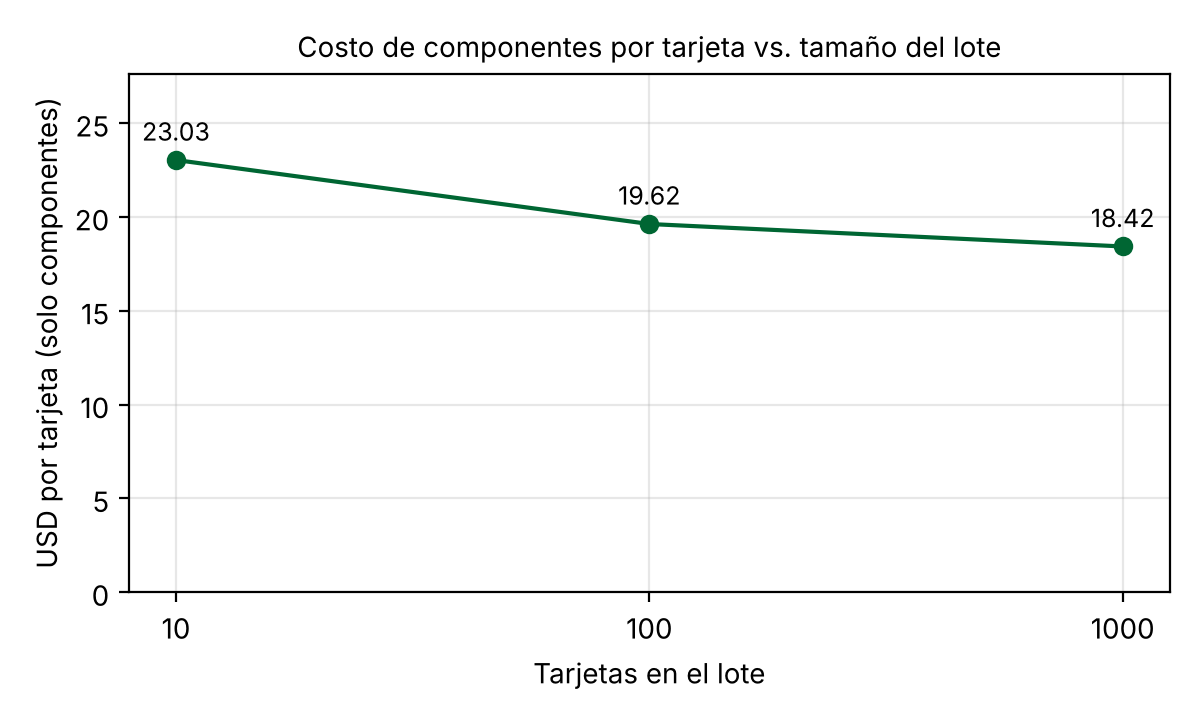
\includegraphics[width=0.8\textwidth]{img/costo_por_tarjeta.png}
\caption{Costo de componentes por tarjeta frente al tamaño del lote.}
\end{figure}

\paragraph{Análisis.} El costo por tarjeta baja de aproximadamente 23{,}0 a 18{,}4~USD de 10 a 1000 tarjetas (cerca de 20~\%). La reducción es moderada porque el costo está dominado por el microcontrolador y las dos memorias, cuyos precios por escalón cambian poco, y porque el último escalón publicado se aplica a cantidades mayores (criterio conservador). El STM32H753IIT6 y las memorias suponen la mayor parte del costo. Alrededor de un 35~\% del costo por tarjeta proviene de precios \textbf{estimados} (SDRAM, cristal, pasivos sin cotizar y conectores genéricos); el eMMC aparece sin stock en la fuente usada, y la SDRAM está en \emph{Last Time Buy}, de modo que la disponibilidad real es un riesgo de costo. Los precios no necesariamente bajan con la cantidad: por ejemplo, SDRAM y los precios con un solo escalón se mantuvieron constantes.

\scriptsize
\setlength{\tabcolsep}{3pt}
\renewcommand{\arraystretch}{1.15}
\begin{longtable}{|>{\raggedright\arraybackslash}p{0.5cm}|>{\raggedright\arraybackslash}p{2.3cm}|>{\raggedright\arraybackslash}p{1.0cm}|>{\raggedright\arraybackslash}p{1.2cm}|>{\raggedright\arraybackslash}p{1.2cm}|>{\raggedright\arraybackslash}p{1.3cm}|>{\raggedright\arraybackslash}p{1.3cm}|>{\raggedright\arraybackslash}p{1.4cm}|>{\raggedright\arraybackslash}p{1.5cm}|>{\raggedright\arraybackslash}p{2.2cm}|}
\hline
\textbf{\#} & \textbf{Designadores} & \textbf{Pzs/tarjeta} & \textbf{USD u. (10)} & \textbf{USD u. (100)} & \textbf{USD u. (1000)} & \textbf{Costo (10)} & \textbf{Costo (100)} & \textbf{Costo (1000)} & \textbf{Estado del precio} \\ \hline
\endfirsthead
\hline
\textbf{\#} & \textbf{Designadores} & \textbf{Pzs/tarjeta} & \textbf{USD u. (10)} & \textbf{USD u. (100)} & \textbf{USD u. (1000)} & \textbf{Costo (10)} & \textbf{Costo (100)} & \textbf{Costo (1000)} & \textbf{Estado del precio} \\ \hline
\endhead
1 & U1 & 1 & 8.0151 & 6.5870 & 6.5870 & 80.15 & 658.70 & 6587.00 & Cotizado \\ \hline
2 & *1 & 1 & 4.6209 & 4.2064 & 3.5938 & 46.21 & 420.64 & 3593.80 & Cotizado (sin stock) \\ \hline
3 & U2 & 1 & 4.8816 & 4.8816 & 4.8816 & 48.82 & 488.16 & 4881.60 & ESTIMADO \\ \hline
4 & U3 & 1 & 0.8819 & 0.6642 & 0.5901 & 8.82 & 66.42 & 590.10 & Cotizado \\ \hline
5 & U4 & 1 & 0.5379 & 0.4006 & 0.3511 & 5.38 & 40.06 & 351.10 & Cotizado \\ \hline
6 & Y1 & 1 & 0.5644 & 0.4321 & 0.4321 & 5.64 & 43.21 & 432.10 & ESTIMADO (variante) \\ \hline
7 & C1, C6 & 2 & 0.0240 & 0.0132 & 0.0080 & 0.48 & 2.64 & 16.00 & Cotizado \\ \hline
8 & R1 & 1 & 0.0340 & 0.0256 & 0.0256 & 0.34 & 2.56 & 25.60 & Cotizado \\ \hline
9 & R6, R7 & 2 & 0.0340 & 0.0256 & 0.0256 & 0.68 & 5.12 & 51.20 & ESTIMADO (proxy) \\ \hline
10 & R2, R3, R4, R5 & 4 & 0.0256 & 0.0256 & 0.0256 & 1.02 & 10.24 & 102.40 & ESTIMADO (proxy) \\ \hline
11 & C2, C5 & 2 & 0.0500 & 0.0200 & 0.0120 & 1.00 & 4.00 & 24.00 & ESTIMADO \\ \hline
12 & C3, C4 & 2 & 0.1000 & 0.0500 & 0.0300 & 2.00 & 10.00 & 60.00 & ESTIMADO \\ \hline
13 & C7 & 1 & 0.1500 & 0.0800 & 0.0500 & 1.50 & 8.00 & 50.00 & ESTIMADO \\ \hline
14 & J1 & 1 & 0.7446 & 0.7423 & 0.6976 & 7.45 & 74.23 & 697.62 & Cotizado (RS, SGD) \\ \hline
15 & J2 (J\_EPS) & 3 & 0.0800 & 0.0500 & 0.0300 & 2.40 & 15.00 & 90.00 & ESTIMADO \\ \hline
16 & J3 (J\_COIL\_X) & 2 & 0.0800 & 0.0500 & 0.0300 & 1.60 & 10.00 & 60.00 & ESTIMADO \\ \hline
17 & J4 (J\_COIL\_Y) & 2 & 0.0800 & 0.0500 & 0.0300 & 1.60 & 10.00 & 60.00 & ESTIMADO \\ \hline
18 & P1 (J\_PAYLOAD) & 5 & 0.0800 & 0.0500 & 0.0300 & 4.00 & 25.00 & 150.00 & ESTIMADO \\ \hline
19 & P2 (J\_CAMERA) & 16 & 0.0500 & 0.0300 & 0.0300 & 8.00 & 48.00 & 480.00 & ESTIMADO \\ \hline
20 & P3 (J\_TELEM) & 4 & 0.0800 & 0.0500 & 0.0300 & 3.20 & 20.00 & 120.00 & ESTIMADO \\ \hline
\end{longtable}
\normalsize
\captionof{table}{Costo por componente y lote (USD).}

\tiny
\setlength{\tabcolsep}{3pt}
\renewcommand{\arraystretch}{1.15}
\begin{longtable}{|>{\raggedright\arraybackslash}p{1.5cm}|>{\raggedright\arraybackslash}p{3.6cm}|>{\raggedright\arraybackslash}p{2.3cm}|>{\raggedright\arraybackslash}p{8.6cm}|}
\hline
\textbf{Clave} & \textbf{Componente} & \textbf{Estado} & \textbf{Fuente} \\ \hline
\endfirsthead
\hline
\textbf{Clave} & \textbf{Componente} & \textbf{Estado} & \textbf{Fuente} \\ \hline
\endhead
STM32 & STM32H753IIT6 & Cotizado & LCSC C146558 (\url{https://www.lcsc.com/product-image/C146558.html}). Referencia; DigiKey/TME muestran 0 o poco stock. \\ \hline
EMMC & EMMC04G-M627-A01 (Kingston) & Cotizado (sin stock) & LCSC C577446 (\url{https://www.lcsc.com/product-image/C577446.html}). Aparece sin stock: disponibilidad PENDIENTE. \\ \hline
SDRAM & MT48LC4M16A2P-6A (Micron) & ESTIMADO & DigiKey ES MT48LC4M16A2P-6A IT:J TR, 4,52 EUR sin IVA, un solo escalón visible (\url{https://www.digikey.com/en/products/detail/micron-technology-inc/MT48LC4M16A2P-6A-IT-J-TR/4315481}). Estado 'Last Time Buy' (fecha 30/06/2026 ya vencida): disponibilidad PENDIENTE; se aplica el mismo precio a los 3 lotes. \\ \hline
ISO & ISO7741DWR (TI) & Cotizado & LCSC C571196 (\url{https://www.lcsc.com/product-image/C571196.html}). Otros distribuidores muestran precios mayores (p.ej. 2,57 EUR en DigiKey DE sin stock). \\ \hline
DRV & DRV8833PWPR (TI) & Cotizado & LCSC C50506 (\url{https://www.lcsc.com/product-image/C50506.html}). DigiKey/Mouser muestran 1,68-2,34 USD. \\ \hline
XTAL & ABM3B-25.000MHZ-B4U-T (Abracon) & ESTIMADO (variante) & Sin cotización de la referencia exacta. Se usa como proxy la variante ABM3B-25.000MHZ-B2-T en LCSC C596875 (\url{https://www.lcsc.com/product-image/C596875.html}). \\ \hline
C100N & GRM155R71C104KA88D (Murata) 0,1 uF 0402 & Cotizado & DigiKey 490-3261-1-ND vía OEMsTrade (\url{https://www.oemstrade.com/search/grm155r71c104ka88d%200402-104k%20pb-free}). \\ \hline
R10K & ERJ3EKF1002V (Panasonic) 10 kOhm 0603 & Cotizado & DigiKey P10.0KHCT-ND (\url{https://www.digikey.com/en/products/detail/panasonic-electronic-components/ERJ-3EKF1002V/196066}). Solo se ven 3 escalones; se mantiene el último. \\ \hline
R\_GEN & Resistencias 33 ohm / 4,7 kohm 0603 1 \% & ESTIMADO (proxy) & Sin cotización de la referencia exacta; se usa el precio de la serie ERJ3EKF (ERJ3EKF1002V). \\ \hline
C\_PF & Condensador 16 pF C0G 0402 & ESTIMADO & Sin cotización. Estimación del equipo; reemplazar al definir la referencia exacta. \\ \hline
C\_2U2 & Condensador 2,2 uF (VCAP) & ESTIMADO & Sin cotización. Estimación del equipo; reemplazar al definir la referencia exacta. \\ \hline
C\_10U & Condensador 10 uF & ESTIMADO & Sin cotización. Estimación del equipo; reemplazar al definir la referencia exacta. \\ \hline
J\_SWD & Molex 53259-0429 (4 pines, 3,5 mm) & Cotizado (RS, SGD) & RS 602-1299, paquete de 10 (\url{https://sg.rs-online.com/web/p/pcb-headers/6021299}). Escalones 10-40, 50-240, 250-740, 750-2240, 2250+. \\ \hline
HDR\_PIN & Cabecera genérica, precio por pin & ESTIMADO & Los conectores J\_EPS, J\_COIL\_X/Y, J\_PAYLOAD, J\_CAMERA y J\_TELEM son símbolos genéricos sin referencia comercial; se estima por pin. \\ \hline
\end{longtable}
\normalsize
\captionof{table}{Fuentes de precio y estado de cada cotización.}

%%%%%%%%%%%%%%%%%%%%%%%%%%%%%%%%%%%%%%%%%%%%%%%%%%%%%%%%%%%%%%%%
\section{Organización del repositorio}\label{sec:repo}

\begin{itemize}
    \item \texttt{Lab04/Esquematicos/PCB2\_OBC\_ADCS/}: proyecto Altium y hojas esquemáticas.
    \item \texttt{Lab04/Esquematicos/2\_Libraries/}: librerías propias.
    \item \texttt{Lab04/Esquematicos/3\_Datasheets/}: hojas de datos (faltan las indicadas en la Sección~4).
    \item \texttt{Lab04/Calculos\_BOM/}: libro de cálculo con BOM, costos y matriz.
    \item \texttt{Lab04/PDF\_Esquematicos/}: esquemáticos en PDF.
    \item \texttt{Lab04/Validacion/}: capturas del ERC.
    \item \texttt{Lab04/Informe/}: este informe.
    \item \texttt{README.md}: integrantes, versión de Altium y cómo abrir el proyecto.
\end{itemize}

%%%%%%%%%%%%%%%%%%%%%%%%%%%%%%%%%%%%%%%%%%%%%%%%%%%%%%%%%%%%%%%%
\section{Conclusiones}
\begin{itemize}
    \item La estructura jerárquica con \emph{signal harnesses} funciona y los errores de conectividad entre hojas (harness sin tipo, designadores duplicados, nombre de red duplicado) se resolvieron.
    \item El esquemático \textbf{no está completo}: SDRAM, eMMC y cámara no están conectadas al microcontrolador, el aislador no cubre las cuatro señales PWM y el lado aislado no tiene alimentación. Estos puntos se documentan como desviaciones y deben cerrarse antes del enrutamiento.
    \item Los cálculos de \emph{pull-ups} I\textsuperscript{2}C cumplen; el del cristal HSE evidencia una discrepancia que debe corregirse.
    \item El costo estimado de componentes es de unos 23~USD por tarjeta en lote de 10 y 18~USD en lote de 1000, con una parte considerable estimada y con riesgos de disponibilidad.
    \item Quedan pendientes la revisión manual, las directivas \emph{Parameter Set} y la verificación documentada de símbolos y huellas.
\end{itemize}

\begin{thebibliography}{99}
\bibitem{nasa_sst} NASA, \textit{State-of-the-Art Small Spacecraft Technology}, 2026. (Referencia heredada de la versión anterior; verificar el capítulo citado.)
\bibitem{jlc} JLCPCB, \textit{PCB Capabilities}, consultado el 27/10/2026. \url{https://jlcpcb.com/capabilities/pcb-capabilities}
\bibitem{jlcbga} JLCPCB, \textit{BGA Design Guidelines}, consultado el 27/10/2026. \url{https://jlcpcb.com/help/article/243-BGA-Design-Guidelines---PCB-Layout-Recommendations-for-BGA-packages}
\bibitem{lcsc} LCSC Electronics, fichas de producto C146558, C577446, C571196, C50506 y C596875, consultadas el 27/10/2026.
\bibitem{digikey} DigiKey, fichas de MT48LC4M16A2P-6A IT:J TR, ISO7741DWR, ERJ-3EKF1002V y GRM155R71C104KA88D, consultadas el 27/10/2026.
\bibitem{ipc} IPC-2221, \textit{Generic Standard on Printed Board Design}.
\end{thebibliography}

\appendix
\section{Esquemáticos completos}
Se anexan las seis hojas del PDF exportado del proyecto (\texttt{Top\_Level}, \texttt{U\_OBC\_Core} --- tres partes del microcontrolador y lógica asociada ---, \texttt{U\_Mass\_Storage}, \texttt{U\_ADCS\_Isolated}, \texttt{U\_Interfaces\_Connectors} y el \emph{Board Stack Report}).

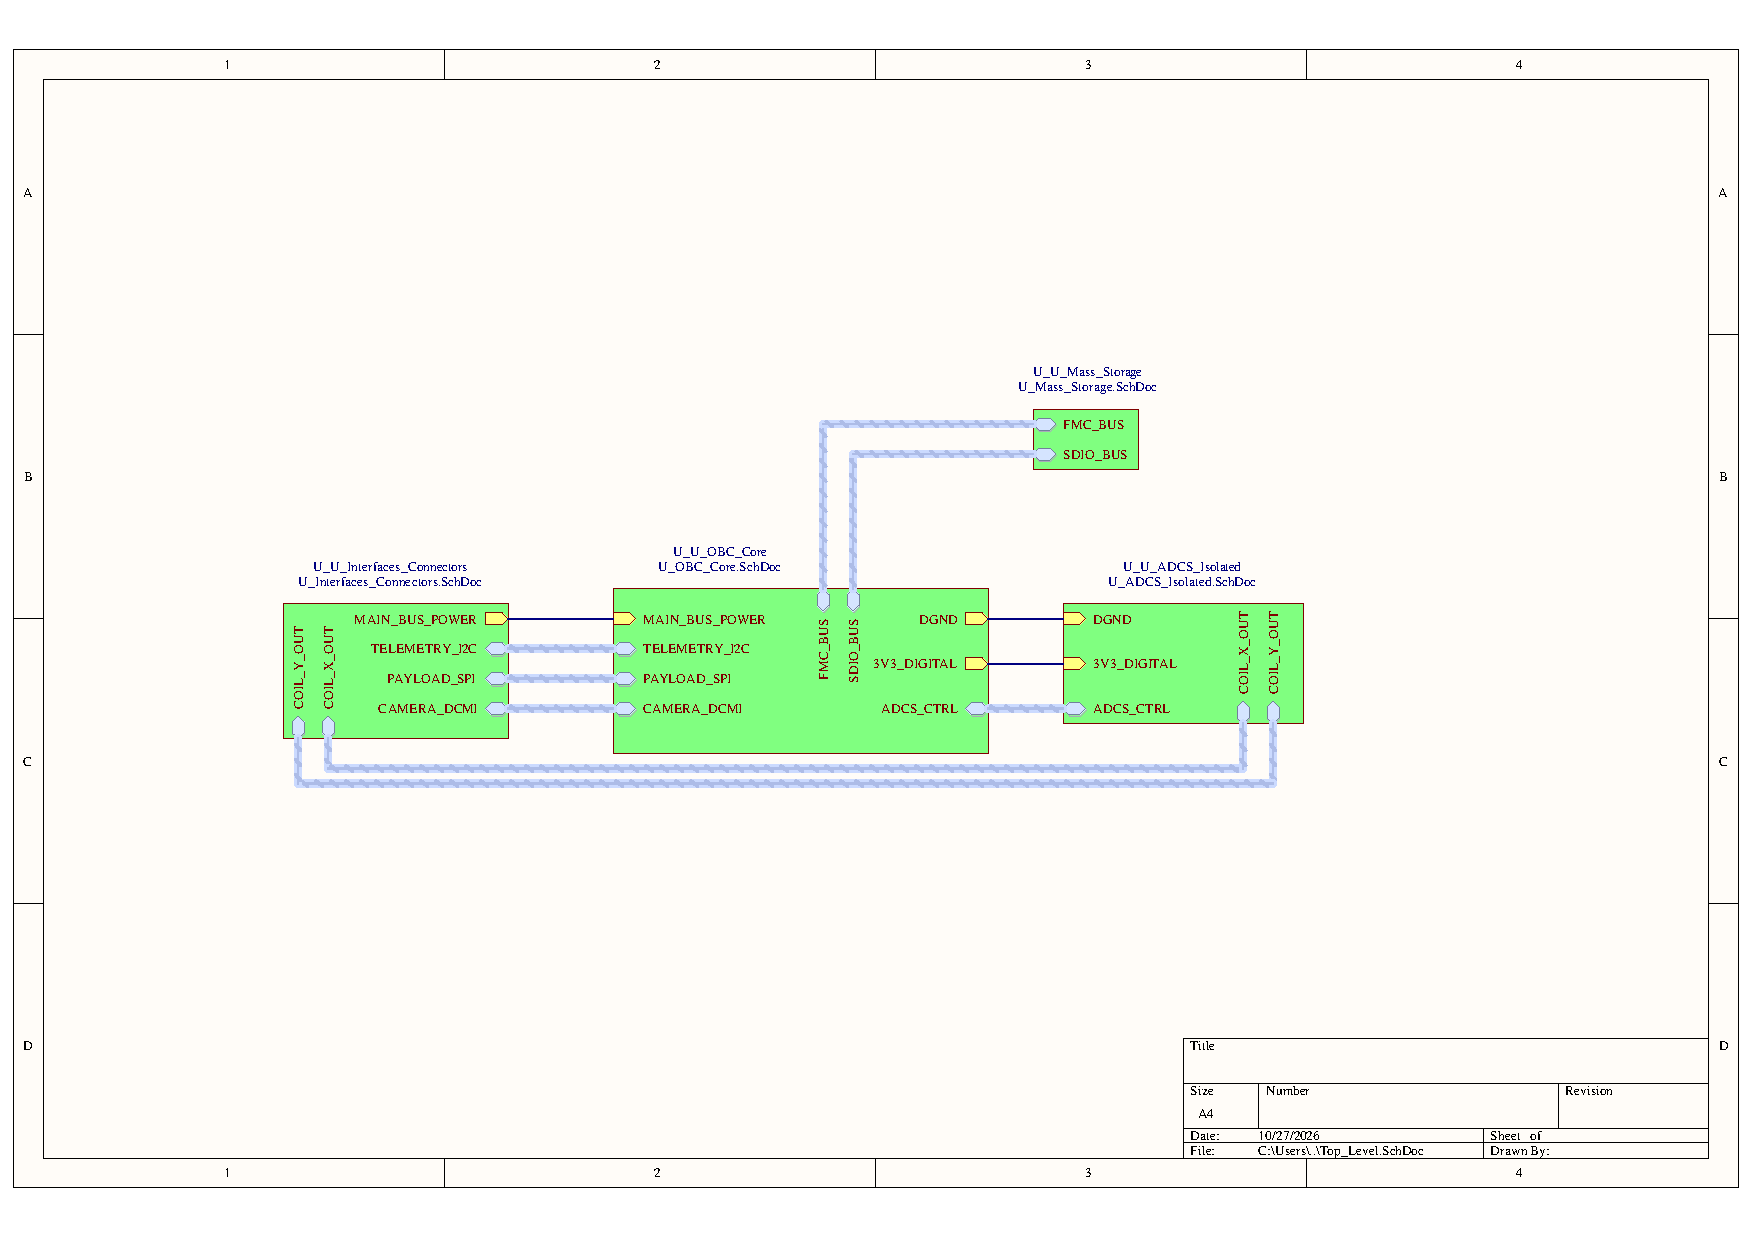
\includepdf[pages=-,landscape=false,pagecommand={},scale=0.95]{img/Esquematico_P4.pdf}

\end{document}
